\documentclass[10pt,letterpaper]{article}
\usepackage[margin=1in]{geometry}
\usepackage[latin1]{inputenc}
\usepackage{amsmath}
\usepackage{amsfonts}
\usepackage{amssymb}
\usepackage{graphicx}
\usepackage{hyperref}
\usepackage[nohyperlinks]{acronym}
\usepackage{float}
\usepackage{subcaption}
\usepackage{pdflscape}
\usepackage{pdfpages}
\usepackage{array}
\usepackage{booktabs}
\usepackage[round]{natbib}
\usepackage{setspace}


\bibliographystyle{plainnat}


\newcommand{\SiIV}{Si\,\textsc{iv}~1403\,\AA}
\newcommand{\HeII}{He\,\textsc{ii}~304\,\AA}
\newcommand{\OIII}{O\,\textsc{iii} 703.87\,\AA}

\newcommand{\tilewidth}{0.25\textwidth}

\newcommand{\TR}{\ac{TR}}
\newcommand{\EE}{\ac{EE}}
\newcommand{\EEs}{\acp{EE}}
\newcommand{\CT}{\ac{CT}}
\newcommand{\CTIS}{\ac{CTIS}}
\newcommand{\MOSES}{\ac{MOSES}}
\newcommand{\ESIS}{\ac{ESIS}}
\newcommand{\EUV}{\ac{EUV}}
\newcommand{\FOV}{\ac{FOV}}
\newcommand{\NN}{\ac{NN}}
\newcommand{\NNs}{\acp{NN}}
\newcommand{\CNN}{\ac{CNN}}
\newcommand{\CNNs}{\acp{CNN}}
\newcommand{\SMART}{\ac{SMART}}
\newcommand{\SAA}{\ac{SAA}}
\newcommand{\CINN}{\ac{CINN}}
\newcommand{\CINNs}{\acp{CINN}}
\newcommand{\DIN}{\ac{DIN}}
\newcommand{\SPIN}{\ac{SPIN}}
\newcommand{\IRIS}{\ac{IRIS}}
\newcommand{\CRS}{\ac{CRS}}
\newcommand{\CRSs}{\acp{CRS}}
\newcommand{\GPU}{\ac{GPU}}
\newcommand{\GAN}{\ac{GAN}}
\newcommand{\SNR}{\ac{SNR}}
\newcommand{\PSF}{\ac{PSF}}


\title{\textsc{Progress Report: \\ Neural Networks for Computed Tomography Imaging Spectroscopy of the Solar Atmosphere}}
\author{Roy Smart \\ \url{roy.smart@montana.edu} \\ Montana State University, Department of Physics \\ Bozeman, MT 59717, USA}


\begin{document}


	
	\maketitle
	
%	\doublespacing
	
	\section{Introduction}
	
		The goal outlined in my NESSF17 proposal was to classify \EEs\ \citep{Brueckner1983} in the solar \TR\ according to their 2D spatial structure.
		I proposed to accomplish this goal using two sounding rocket-borne instruments optimized towards observing \EEs, the \MOSES \citep{kankel1}, and the \ESIS.
		\MOSES\ flew successfully in 2006 \citep{fox1} and 2015 \cite{smart1}, and both instruments are planned to fly in 2019.
		These instruments are members of a class of spectrographs known as snapshot imaging spectrographs, which can spectrally-resolve a 2D \FOV\ in a single snapshot, as opposed to imaging spectrographs, such as \IRIS\ \citep{DePontieu2014}, which can only spectrally-resolve a 2D \FOV\ through rastering.
		Snapshot imaging spectrographs are needed to adequately characterize the spatial structure of \EEs, since \EEs\ evolve faster than the rastering timescale of \IRIS \citep{kankel1,DePontieu2014}.
		
		\MOSES\ and \ESIS\ are a type of snapshot imaging spectograph known as a \CTIS \citep{Okamoto:91}, which takes a snapshot of a 2D \FOV\ by simply removing the slit used by imaging spectrographs.
		Without the slit, space and spectrum become confused, so images are taken at several diffraction orders/angles to provide adequate information about the scene.
		These images can be interpreted as a spectrally-resolved 2D scene using \CT\ inversion algorithms, hence the name \CTIS.
		Spectrally-resolving \MOSES\ and \ESIS\ data is an ill-posed inversion problem because they only image in a limited number (3-6) of diffraction orders/angles \citep{kankel1}.
		
		A brute-force approach to addressing this ill-posed inversion problem would be to use a forward model of a \MOSES/\ESIS\ and an a priori model of solar \TR\ spectra to create a dictionary of spectral structures and their corresponding signature on the \CTIS\ detectors.
		This would allow \CTIS\ observations to be matched to entries in this dictionary to recover a spectrally-resolved scene.
		I developed an approximation to the above brute-force approach using \NNs, known as a \CINN.
		This approximation aims to spectrally-resolve \MOSES\ and \ESIS\ observations using thousands of \IRIS\ \SiIV\ spectra as a model of the solar \TR.
		
		\NNs\ are an efficient regression technique for fitting a curve to an arbitrary set of data \citep{ai}, known as the training data.
		Our \CINNs\ are a \NN\ designed to invert a function that maps spectral line parameters to their corresponding signal on the \CTIS\ detectors.
		To accomplish this, we apply a \CTIS\ forward model to a large set of \IRIS\ \SiIV\ spectra and then use the a \NN\ to fit the inverse function.
		The \CTIS\ forward model is spatially invariant, so it is not necessary to make a neural network large enough to invert an entire \CTIS\ image.
		Instead, we can implement a neural network that can invert a single pixel, and then convolve this \NN\ with a \CTIS\ observation to construct a spectrally-resolved image.
		This type of neural network is known as a \CNN\ and is an important optimization that makes this problem tractable on a modern consumer \GPU.
			
		We have completed a simple realization of a \CINN\ for the \MOSES-06 instrument, the \DIN, which reconstructs the Doppler-shift of the \HeII\ spectral line observed by \MOSES-06.
		We found that our implementation of a \DIN\ was more accurate at reconstructing large Doppler velocities than existing \CT\ algorithms.
		However, we also discovered that \CRS\ in the \IRIS\ \SiIV\ observations were confounding the predictive power of our \DIN, motivating the addition of a \IRIS\ despiking routine into our procedure.
		Existing \IRIS\ despiking routines were ill-suited to processing thousands of \IRIS\ observations, because of the need to manually tune these routines for each unique \IRIS\ observation.
		Therefore, we developed our own GPU-accelerated despiking routine designed to provide acceptable automated despiking performance across our \IRIS\ dataset.
		
		For the remainder of my NESSF17 proposal (up to 09-01-18), I plan to introduce numerous improvements to our \IRIS\ data pipeline, including the improved despiking routine, and produce a publication describing the application of our \DIN\ to the \MOSES-06 dataset.
		In my proposed schedule for NESSF18, I will develop and produce a publication on an improved \CINN\ with the capability to reconstruct the full spectral line profile of the \MOSES-06 observation (dubbed a \SPIN), and begin development of a \EE\ classification scheme.
		
	
	\section{NESSF17 Progress Report} 
	
		We presented preliminary results of a \SPIN\ for inverting the \MOSES-06 dataset in Section 2.3 of our NESSF17 proposal.
		An important issue with these results is that they are blurry with respect to the original image.
		It was expected that we could resolve this issue by creating a larger neural network, but it persisted regardless of the network size.
		After more research it was determined that this behavior was due our use of the Euclidean norm as a loss function, the function that measures the fit of the \NN\ to the data.
		This is a well-documented limitation of using the Euclidean norm for image reconstruction \citep{Pathak2016}.
		It was determined that we would require a more sophisticated loss function, which we will discuss further in Section \ref{sec_gan}, but we decided to first try and solve a simpler problem using our existing architecture.
					
		\subsection{Doppler Inversion Network}
		
			\EEs\ are characterized by non-thermal Doppler broadening on the order of 100\,km/s, and/or comparable Doppler shifts of an \TR\ emission line \citep{Dere1989}.
			Therefore, to identify and classify \EEs\ we do not necessarily need to recover the spectral line profile from a \CTIS\ instrument, just the Doppler shift and width of the line profile.
			Solving for these two parameters is simpler than the spectral line profile since they contain less information.
			We modified our \SPIN\ that mapped \MOSES\ observations to spectral line profiles, to a \DIN\ that mapped \MOSES\ observations to the \textit{mean} of a spectral line profile, a measurement of Doppler shift.
			The \DIN\ allows for the extraction of useful plasma parameters while retaining the simplicity of our original method.
			
			Our \DIN\ implementation is a \CNN\ with a 21x1 pixel kernel that is convolved with MOSES observations to calculate the Doppler shift at each pixel.
			Our training dataset consisted of 4.5k \IRIS\ spectra selected for their high \SNR\, and we also constructed a validation dataset containing the same number of images to test our method against a statistical independent sample.
			This kernel size represents a window of $\pm$300\,km/s in MOSES pixels, providing a healthy margin around the typical 100\,km/s size of \EEs \citep{Dere1994}.
			For this kernel size, we developed two networks: a \textit{Test} network with 1k free parameters, and a \textit{Final} network with 800k free parameters.
			In Table \ref{nn_table} we have listed some important properties of these two networks, along with some qualitative measures of their performance.
			This was done as a preliminary test of the quality of the reconstructed results, as a function of network complexity.
			We can see that both networks were able to achieve an RMS velocity error better than the theoretical resolution of MOSES (29\,km/s).
			Also we will point out that the training time was very short, only 15 minutes for the Final network.
			This performance is possible thanks to \GPU\ implementations of our \NN\ libraries.
			
			\begin{table}[t!]
				
				\centering
				\begin{tabular}{| l | c c |}
					\hline
					& Test & Final \\ \hline
					Free Parameters & 1.2k & 836k \\
					Training Images & 4.5k & 4.5k \\				
					Training time (min) & 3 & 15 \\ 
					RMS error (km/s) & 12.7 & 10.3 \\
					Pearson's $r$ & 0.500 & 0.701 \\ \hline				
				\end{tabular}					
				\caption{Description of the characteristics and results of two neural networks tested for this progress report. More comprehensive results from the Final network are presented in later figures.}
				\label{nn_table}
				
			\end{table}
		
			\begin{figure*}[t!]
				\centering
				\begin{subfigure}[t]{0.45\textwidth}
					\centering
					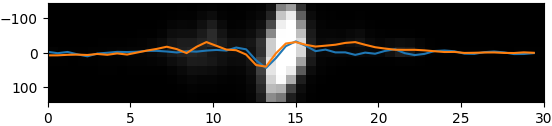
\includegraphics[width=\textwidth]{fig/doppler_1182}
				\end{subfigure}
				~ 
				\begin{subfigure}[t]{0.45\textwidth}
					\centering
					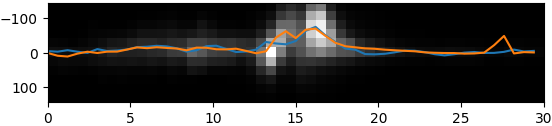
\includegraphics[width=\textwidth]{fig/doppler_1225}
				\end{subfigure}
				~ 
				\begin{subfigure}[t]{0.45\textwidth}
					\centering
					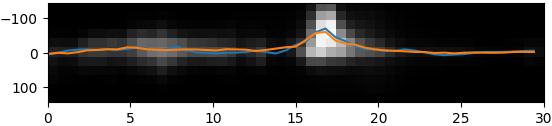
\includegraphics[width=\textwidth]{fig/doppler_1263}
				\end{subfigure}
				~ 
				\begin{subfigure}[t]{0.45\textwidth}
					\centering
					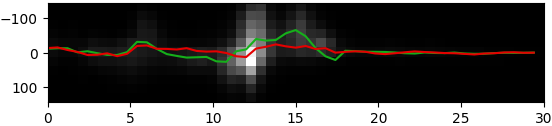
\includegraphics[width=\textwidth]{fig/doppler_1343}
				\end{subfigure}
				\caption{Examples of Doppler inversions. Each image is an IRIS \SiIV\ spectrum rebinned into \MOSES\ resolution. The vertical axis is wavelength (km/s) and the horizontal axis is space (arcsec). The true line center is plotted in green, and the reconstructed line center is plotted in red.}
				\label{dopp_ex}
			\end{figure*}
			
			In Figure \ref{dopp_ex} we have provided a few validation examples of our method, where we have plotted the reconstructed Doppler velocity along with the true velocity for comparison. 
			We chose to show these validation examples since they demonstrated reasonably-high Doppler velocities, characteristic of some types of \EEs.
			We can see that in areas of high signal the network does reasonably well at reproducing the true Doppler shift, while in areas of low signal the Doppler shift is underestimated.
			We anticipate that the despiking procedure outlined in Section \ref{sec_dspk} will improve results in these low-signal areas, since spikes are more effective at changing the estimated Doppler shift in these areas.
			
			\begin{figure*}[t!]
				\centering
				\begin{subfigure}[t]{0.45\textwidth}
					\centering
					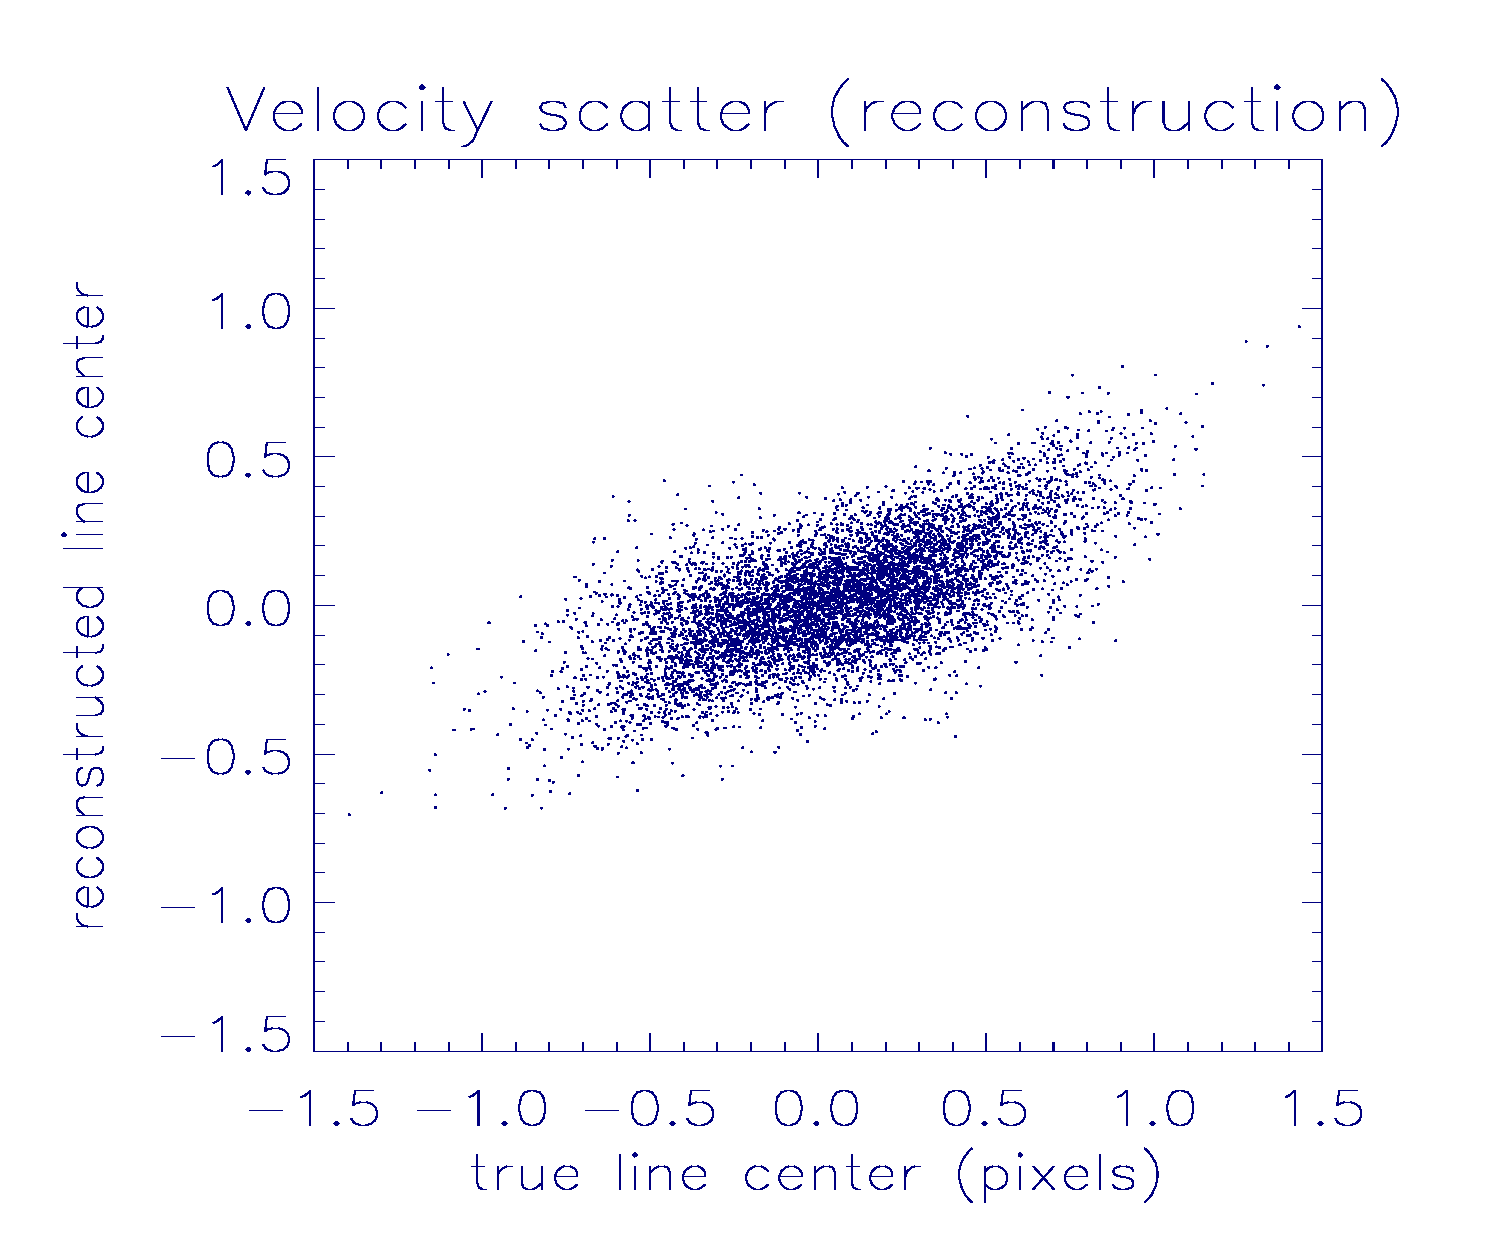
\includegraphics[width=\textwidth]{fig/smart_hist}
					\caption{SMART}
					\label{smart_hist}
				\end{subfigure}%
				~ 
				\begin{subfigure}[t]{0.45\textwidth}
					\centering	
					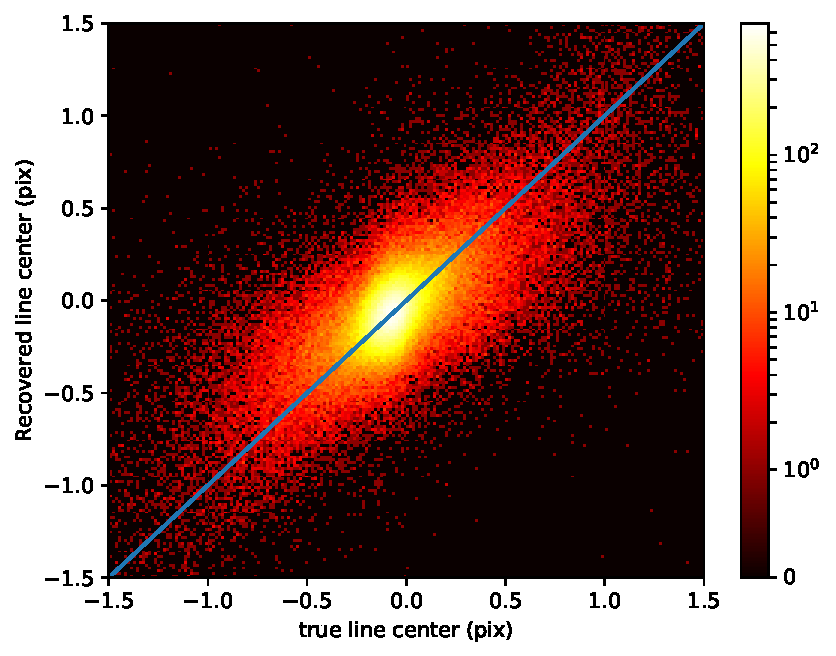
\includegraphics[width=\textwidth]{fig/linearity}
					\caption{DIN}
					\label{din_hist}
				\end{subfigure}
				\caption{Reconstructed vs. true Doppler velocity using both the standard SMART algorithm (applied to SUMER \OIII\ raster)\citep{Kankelborg2004}, and the CINN algorithm (applied to our \IRIS\ \SiIV\ validation dataset). 
					Figure \ref{smart_hist} is a scatterplot of the reconstructed velocity vs. true velocity for every pixel in the SUMER raster. 
					Figure \ref{din_hist} is a column-normalized histogram (where each column is an independent, normalized distribution) with the same axes as Figure \ref{smart_hist}. 
					Plotted in red is the line of perfect reconstruction.
					}
				\label{dopp_hist}
			\end{figure*}

			Currently, the \SMART\citep{fox1} serves as the de facto standard algorithm for MOSES spectral line profile inversions.
			In Figure \ref{smart_hist} we can see an important test of this algorithm, the Doppler velocity (mean) of the reconstructed spectral line profile, compared to the mean of the original (or true) line profile.
			This test can be represented as a scatterplot since it consisted of applying \SMART\ to a single SUMER raster.
			
			In Figure \ref{din_hist} we present an analogue of Figure \ref{smart_hist} for the \DIN\ calculated using our validation dataset.
			Since the validation dataset is so large, it would be poorly represented as a scatterplot, so we present it as a column-normalized 2D histogram, where each bin of the histogram has been divided by the sum of its column.
			This presentation demonstrates the probability of accurately reconstructing the Doppler velocity as a function of the true Doppler velocity.
			We have also plotted the line of perfect reconstruction, if the algorithm were perfect, all the probability would be in pixels under this line.
			We calculated Pearson's $r$ of this histogram for both our Test and Final networks, and were able to verify that the addition of more free parameters corresponded to significant improvement in the performance of the network under this metric.
			
			\SMART\ has a systematic tendency to underestimate the reconstructed velocity, a well studied property of this algorithm \citep{Fox2011,Rust2017}.
			We can see that the \DIN\ does a much better job, on average, of correctly estimating the velocity, however there is still significant underestimation of velocity.
			We think that this underestimation is at least partially due to \CRSs\ in both the training and validation datasets, which we will discuss in Section \ref{sec_dspk}.
			For now, we consider these results exciting verification of our method, since the \DIN\ method allows for more accurate reconstructions of high-velocity events such as \EEs.		
						
		\subsection{Despiking Training Data}	\label{sec_dspk}	
			
			\begin{figure}[b!]
	
				\renewcommand{\arraystretch}{0}
				\setlength{\tabcolsep}{0pt}
				\begin{tabular}{m{0.1\textwidth} m{\tilewidth} m{\tilewidth} m{\tilewidth} @{}m{0pt}@{}}
					& \centering IRIS Level 2 & \centering \texttt{iris\_prep\_despike.pro} & \centering Our Method & \\[5mm]
					Region 1 & 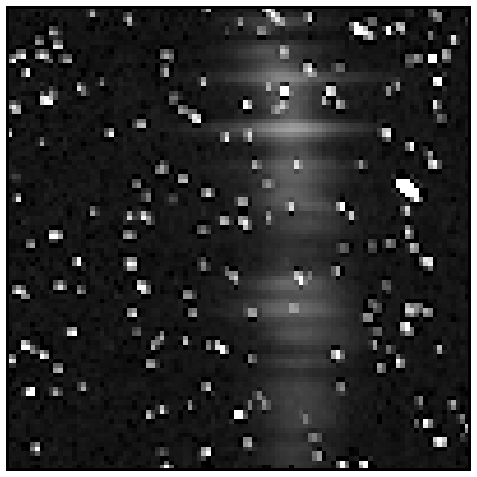
\includegraphics[width=\tilewidth]{fig/orig_1} & 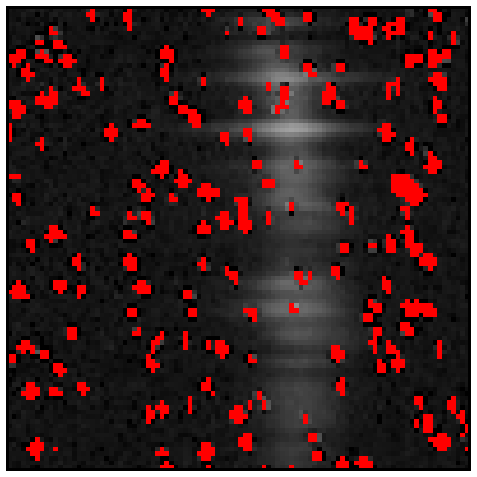
\includegraphics[width=\tilewidth]{fig/despike_1} & 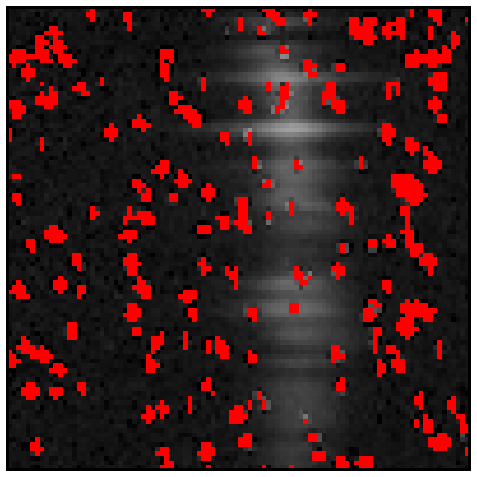
\includegraphics[width=\tilewidth]{fig/dspk_1} & \\
					Region 2 & 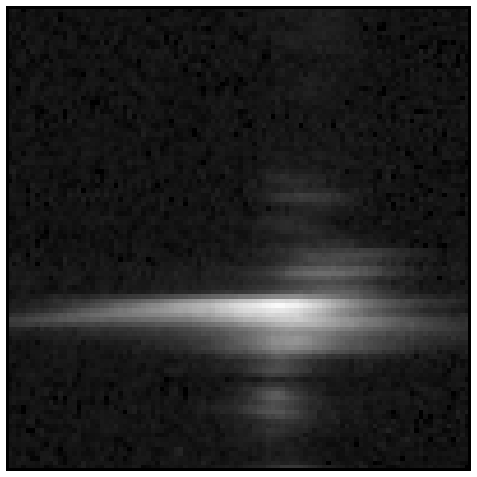
\includegraphics[width=\tilewidth]{fig/orig_2} & 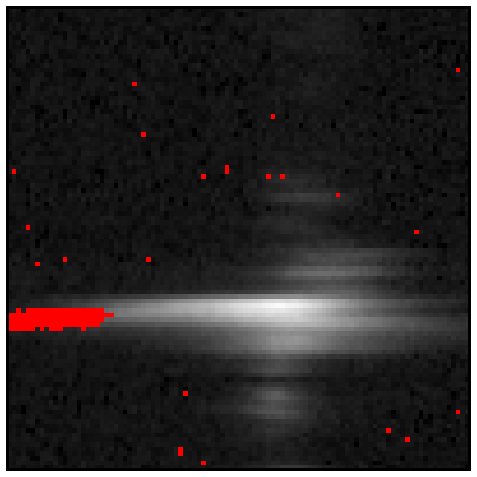
\includegraphics[width=\tilewidth]{fig/despike_2} & 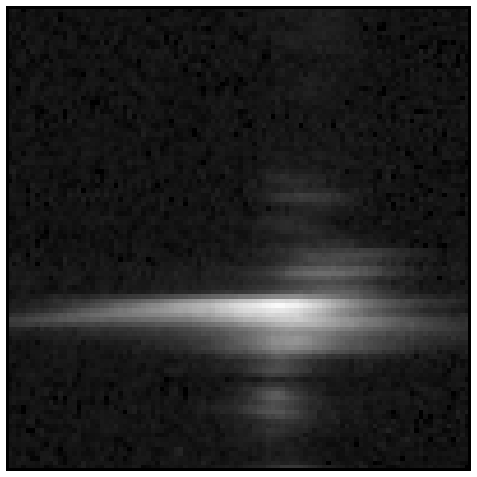
\includegraphics[width=\tilewidth]{fig/dspk_2} & \\
				\end{tabular}
				
				\caption{An example of both the standard despiking algorithm and our spike identification algorithm applied to an IRIS \SiIV\ observation gathered at 07:24:26 on 06-16-2015.
					Pixels containing spikes are marked red by each algorithm.
					We present cutouts from frames 24 and 50 to demonstrate how susceptible each algorithm is to false spike identifications. 
					The frame on the top row was taken inside the \SAA, and provides examples of many types of spikes intended to show the false negatives identified by each algorithm.
					The frame on the bottom row is an example of an \EE, and serves as an example of the false positives identified by each algorithm.}
				
				\label{dspk_ex}
				
			\end{figure}
			
			\begin{figure}[t!]
				\centering
				\begin{subfigure}[t]{0.288\textwidth}
					\centering
					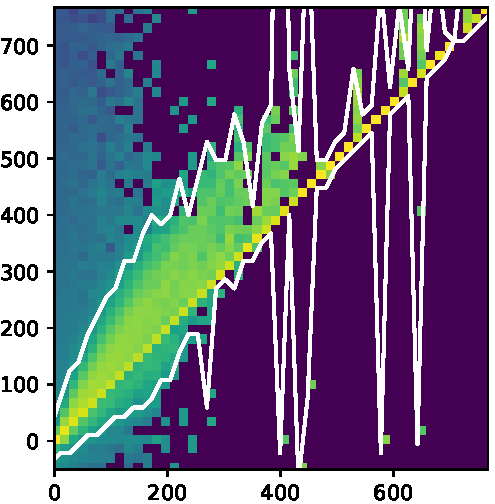
\includegraphics[width=\textwidth]{fig/hist_0}
					\caption{Wavelength}
				\end{subfigure}
				~ 
				\begin{subfigure}[t]{0.288\textwidth}
					\centering
					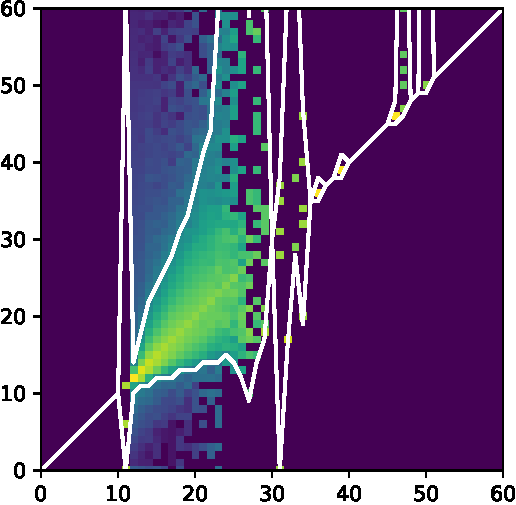
\includegraphics[width=\textwidth]{fig/hist_1}
					\caption{Space}
				\end{subfigure}
				~ 
				\begin{subfigure}[t]{0.288\textwidth}
					\centering
					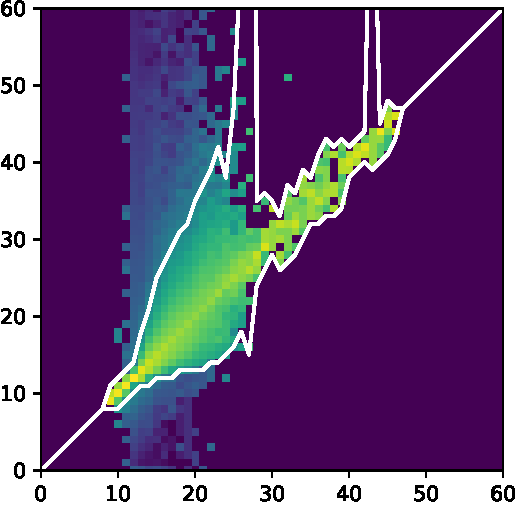
\includegraphics[width=\textwidth]{fig/hist_2}
					\caption{Time}
				\end{subfigure}
				~ 
				\begin{subfigure}[t]{0.079\textwidth}
					\centering
					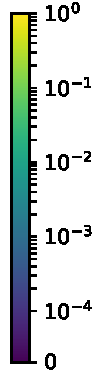
\includegraphics[width=\textwidth]{fig/cbar}
				\end{subfigure}
				
				\caption{Column-normalized histogram of local median intensity along each axis vs. intensity for the observation in Figure \ref{dspk_ex}.
					Each column has been divided by its total to understand the distribution of values about a particular median.
					The 1\% and 99\% thresholds have been plotted in white.
					}
				
				\label{dspk_hist}
				
			\end{figure}
			
			Spikes in IRIS observations are a stochastic process, primarily due to ionospheric particles impacting the CCD detectors \citep{itn15}.
			Removal of spikes in our training dataset is important since the network will become distracted trying to reconstruct the spikes, a futile undertaking.
			This was not considered to be a serious problem during the proposal phase, as there have been several despiking routines written for IRIS.
			However we failed to appreciate how difficult it would be to apply these routines in an automated fashion to a large section of the IRIS \SiIV\ dataset.
			
			There are a multitude of despiking routines available on the IDL SolarSoft libraries, such as \texttt{nospike.pro}, \texttt{array\_despike.pro}, \texttt{iris\_prep\_despike.pro}.
			All these procedures identify spikes using the same method: convolution of some kernel with an image to estimate a local mean and standard deviation, and a hard threshold to exclude pixels some number of standard deviations above the mean.
			This method is often too aggressive in areas of high signal intensity and not aggressive enough in areas of low signal intensity.
			In Figure \ref{dspk_ex}, we can see an example of this behavior: the explosive event in the bottom row has become eroded from \texttt{iris\_prep\_despike.pro}, while many of the spikes in the top row are only partially identified.
			Considering this behavior, to use these procedures we found that we would have to manually tune them for each observation, which would become prohibitive for a training dataset composed of thousands of IRIS observations.
			
			Instead of estimating the mean and standard deviation, our method uses a median-percentile based approach, where pixels are marked as spikes if their value is larger than 99\% (for example) of all other pixels with the same median. 
			This is accomplished by calculating a local median for every pixel in the observation, and then constructing a histogram of local median vs. pixel value for each observation.
			From this histogram, we can then determine the bad pixel threshold as a function of the local median.
			Finally, this procedure was performed independently along each axis (wavelength, space, time) and we required that a pixel must be above the threshold for all three axes to be marked as a spike.
			A visualization of this procedure is presented in Figure \ref{dspk_hist}, where we can see the thresholds of each axis overplotted on the histograms used to perform the despiking seen in Figure \ref{dspk_ex}.		
			We have developed a GPU implementation of this despiking procedure, resulting in code that is at least 10x faster than current methods while being much more discriminatory at avoiding false positives and false negatives.

		
	\section{Remainder of NESSF17 Schedule}
	
		With the exception of exchanging the \SPIN\ development for the \DIN\ development, we are consistent with the schedule given in my NESSF17 proposal, on track for a publication to be submitted before the end date of the proposal period.
		This publication will cover the motivation, implementation, and validation of our \DIN, with applications to the \MOSES-06 dataset.
		We will compare the inversions recovered using the \DIN\ to those calculated using other methods to determine if the \DIN\ is a worthwhile improvement.
		Our inversions of the \MOSES-06 dataset will be available to the public, to support further investigations into this dataset.
		Also, we will release our despiking routine to the public to promote easier analysis of \IRIS\ data and allow other researchers to adapt the code for their needs.
		
		Before the results of our method can be published, we need to make a few improvements to the training data pipeline such as: the despiking procedure discussed in Section \ref{sec_dspk}, a model of the \MOSES-06 passband \citep{Fox2011}, a solar continuum model around \HeII \citep{Fox2011}, and an accurate noise model for the \MOSES-06 detectors \cite{Rust2017}.
		We also need to implement some critical preprocessing steps to the \MOSES-06 dataset such as: \PSF\ deconvolution \citep{Rust2017}, and spectral contamination removal \citep{Parker2016}.
		Additionally, we need to improve our network architecture to include the width of the spectral line profile.
		Finally, our validation tests need to be improved, with \SMART\ applied to the same validation set as the \DIN, and several simple validation tests such as those in \cite{Rust2017}.
	
	\section{NESSF18 Proposal}
	
		We are proposing to continue this research under the NESSF18 solicitation.
		The results we have obtained so far show that our method is superior to current techniques in terms of reconstruction accuracy of Doppler shift.
		We think this merits additional investigation into using \CNN\ techniques to interpret data from \CTIS\ instruments such as \MOSES\ and \ESIS.
		Furthermore, we have made progress in terms of our \CTIS\ analysis tools, but we haven't yet developed any software to address our ultimate goal of classifying \EEs.
		We plan to implement a more sophisticated \SPIN\ during the first half of the NESSF18 proposal period, and to begin work on an \EE\ classifier during the second half of the proposal period.
	
		\subsection{MOSES Inversion GAN} \label{sec_gan}
		
			An exciting advancement in using \CNNs\ for image reconstruction has been the development of \textit{adversial loss} as opposed to the Euclidean loss used by our current networks. 
			This concept is expressed in a new type of \NN\ called a \GAN, developed by \cite{Goodfellow2014}. 
			In this type of network, our current \DIN\ is known as the \textit{generator} network, and its output is an input to the \textit{adversary} network. 
			The adversary network's task is to compare the output image of the generator network to the true image and determine which one was created by the generator network.
			The loss is minimized when the adversary network can't distinguish between the generated image and the true image \cite{Isola2016}.
			This method was recently used for \PSF\ deconvolution of astrophysical images by \cite{Schawinski2017}, the results indicate that this is a powerful technique that is well-suited to our inversion problem.
			
			Our plan is to pursue development of a \GAN\ for a \MOSES\ \SPIN\ after the submitting our publication describing the \DIN.
			We expect the development time should be relatively short considering that we can use the training dataset from the \DIN.
			If this \MOSES\ inversion \GAN\ is shows improvement over our current method, we will publish a short article describing the implementation and results of our approach.
			
		
		\subsection{Explosive Event Classification}
		
			The literature has conducted extensive analyses of \EEs\ using rastering imaging spectrographs, such as \IRIS.
			They identify \EEs\ as an enhancement of the red and/or blue wings of emission lines forming between 20,000K and 250,000K \citep{Moses1994}.
			These events are often spectrally classified into two groups: those with enhancements in both wings and those with enhancement in only one wing \citep{Dere1989}.
			The wings are sometimes displaced from one another by a few thousand kilometers \citep{Dere1994}, indicating a dynamic spatial structure.
			Recently, \cite{Innes2015} interpreted \EEs\ as evidence of  MHD reconnection through the plasmoid instability, however there have been many other explanations for \EEs\ such as: flows along loops \citep{Teriaca2004}, flows along spicules \citep{Wilhelm2000} and plasma ejection and retraction \citep{Huang2014}.
			Presently, it is unclear if \EEs\ can be explained by one physical mechanism, or if multiple mechanisms are required to explain their characteristics.
			
			In our NESSF17 proposal we asked: \textbf{If these events do arise from multiple mechanisms, can we distinguish different types of explosive events by considering their spatial structure?}
			To answer this question, the spectrally-resolved images of the solar \TR\ taken using \MOSES\ and later \ESIS\ will be used to isolate \EEs\ and construct a database of events.
			We will then apply simple \textit{clustering} algorithms, such as $k$-means \citep{Macqueen1967}, to test if \EEs\ can naturally be classified into different groups.
			This is an important first step to see if any obvious classes of \EEs\ can be identified.
			We intend to present preliminary results of our investigation into this method in our NESSF19 progress report.
			
	
	
	\begin{landscape}
		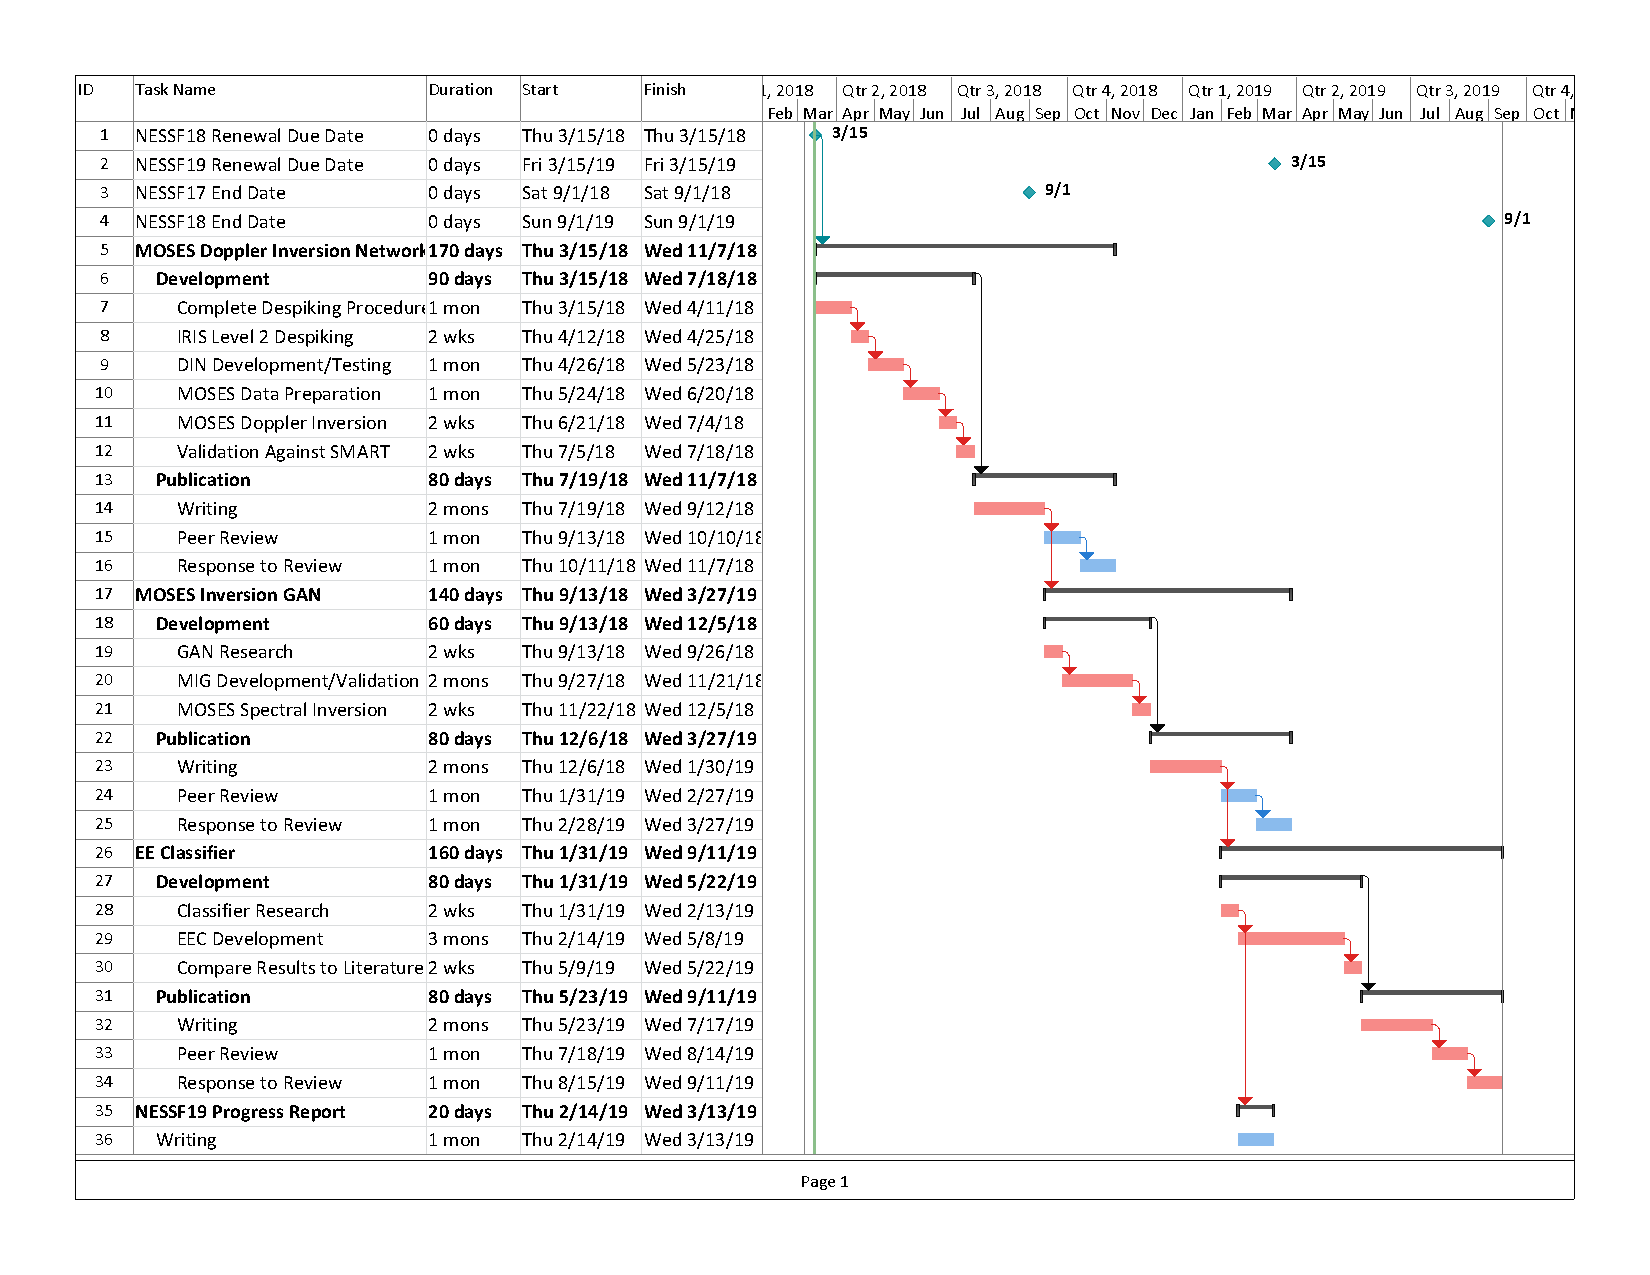
\includepdf[pages=-,landscape=true]{../schedule/NESSF18_schedule}
	\end{landscape}
	
	\bibliography{bib/sources}
	
	\section{List of Acronyms}
	\begin{acronym}
		\acro{TR}{transition region}
		\acro{EE}{explosive event}
		\acro{CT}{computed tomography}
		\acro{CTIS}{computed tomography imaging spectrograph}
		\acro{MOSES}{\textit{Multi-order Solar EUV Spectrograph}}
		\acro{ESIS}{\textit{EUV Snapshot Imaging Spectrograph}}
		\acro{EUV}{extreme ultraviolet}
		\acro{FOV}{field-of-view}
		\acro{NN}{neural network}
		\acro{CNN}{convolutional neural network}
		\acro{SMART}{smooth multiplicative algebraic reconstruction technique}
		\acro{SAA}{South-Atlantic Anamoly}
		\acro{CINN}{CTIS inversion neural network}
		\acro{DIN}{Doppler inversion network}
		\acro{SPIN}{spectral profile inversion network}
		\acro{IRIS}{\textit{Interface Region Imaging Spectrograph}}
		\acro{CRS}{cosmic ray spikes}
		\acro{GPU}{graphics processing unit}
		\acro{GAN}{generative adversarial network}
		\acro{SNR}{signal-to-noise ratio}
		\acro{PSF}{point-spread function}
	\end{acronym}
	
	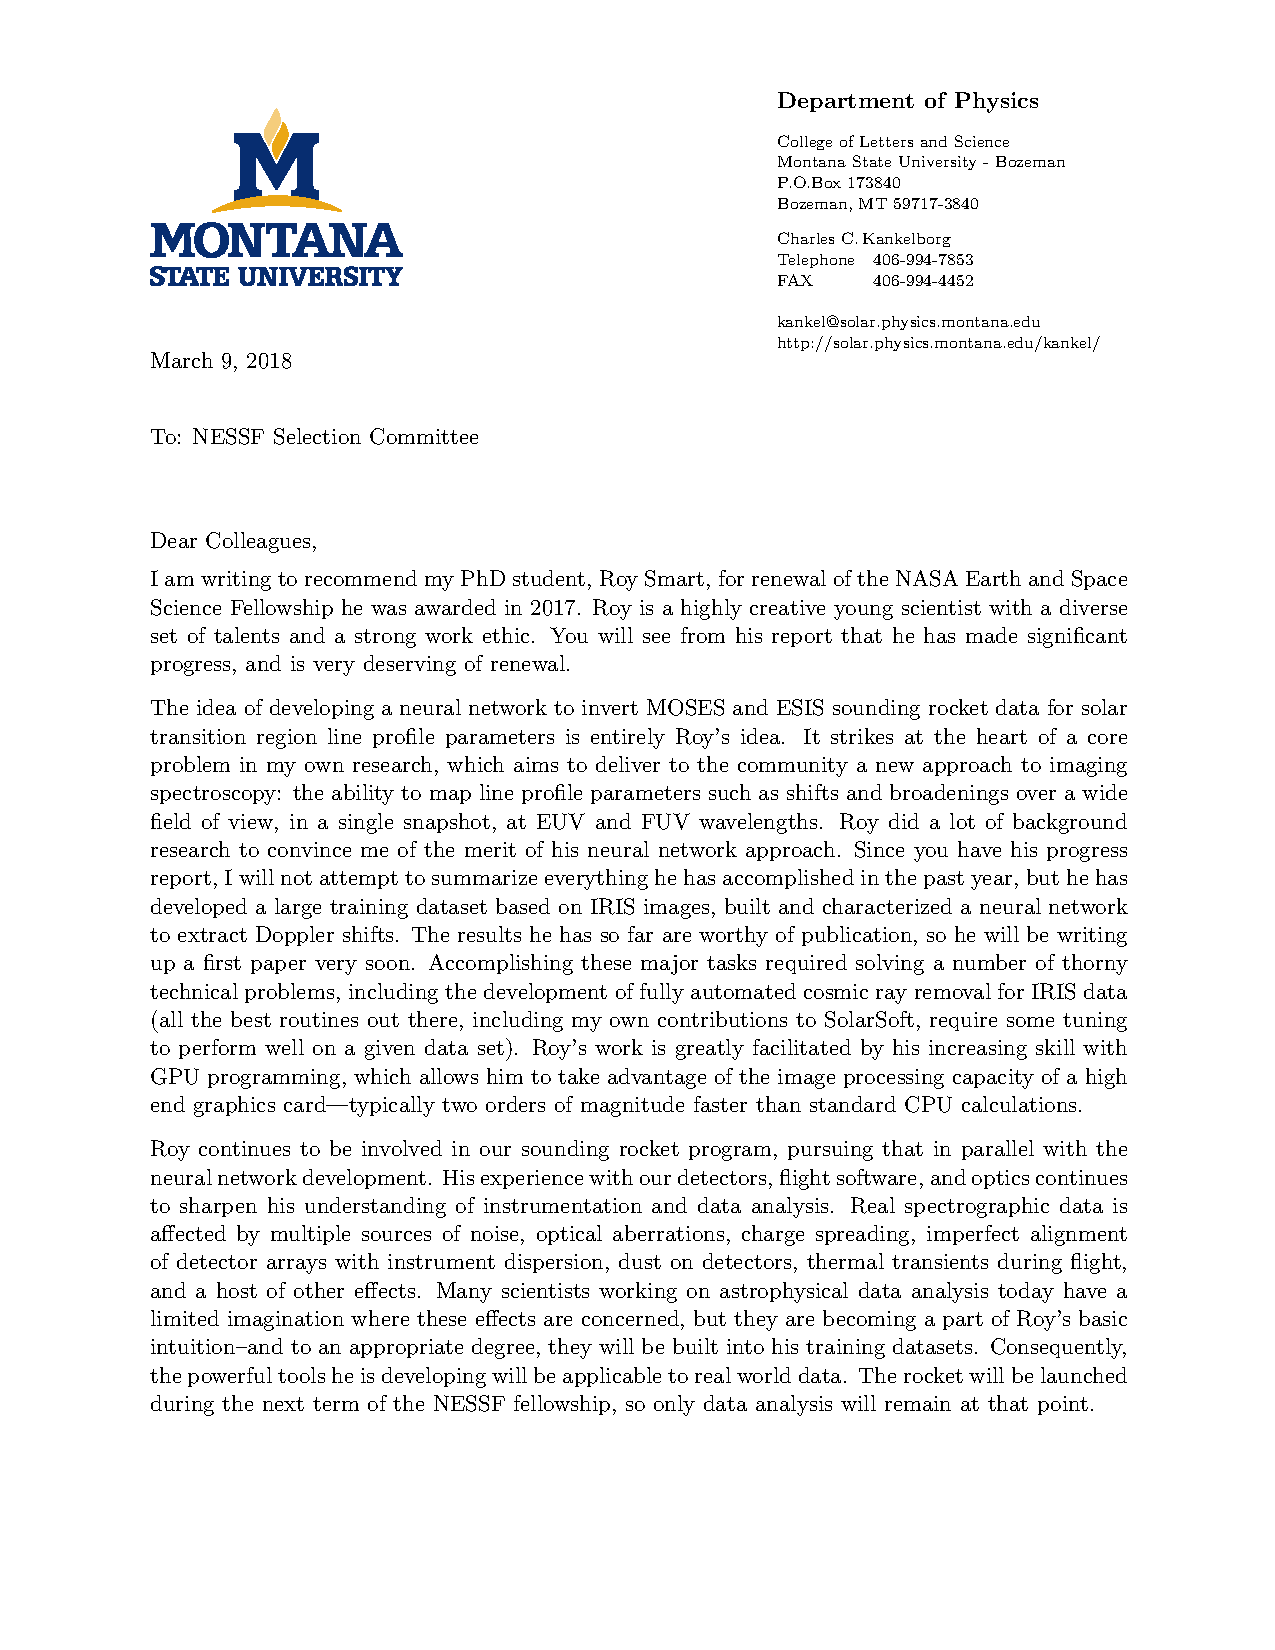
\includepdf[pages=-]{../recommendation/nessf17smartLetter}
	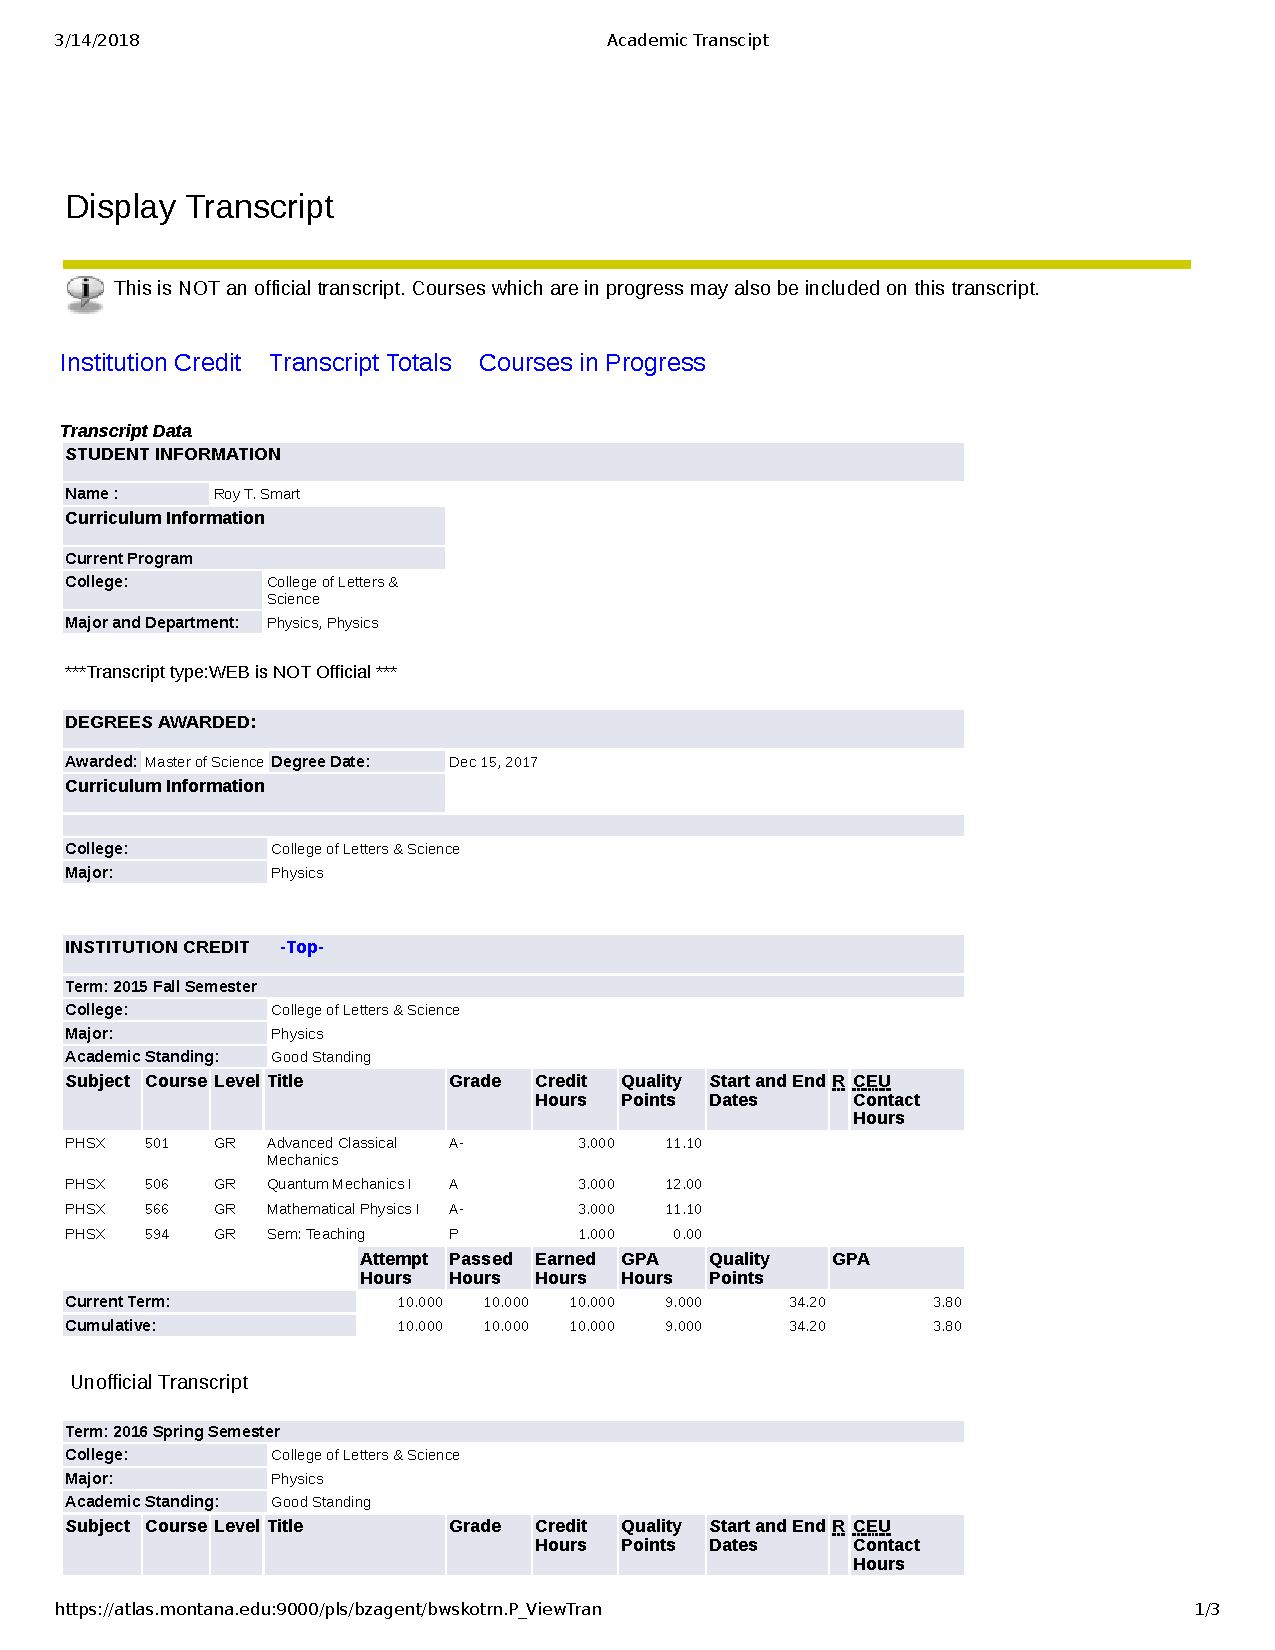
\includepdf[pages=-]{../transcript/transcript}
	
\end{document}